%=======================02-713 LaTeX template, following the 15-210 template==================
%
% You don't need to use LaTeX or this template, but you must turn your homework in as
% a typeset PDF somehow.
%
% How to use:
%    1. Update your information in section "A" below
%    2. Write your answers in section "B" below. Precede answers for all 
%       parts of a question with the command "\question{n}{desc}" where n is
%       the question number and "desc" is a short, one-line description of 
%       the problem. There is no need to restate the problem.
%    3. If a question has multiple parts, precede the answer to part x with the
%       command "\part{x}".
%    4. If a problem asks you to design an algorithm, use the commands
%       \algorithm, \correctness, \runtime to precede your discussion of the 
%       description of the algorithm, its correctness, and its running time, respectively.
%    5. You can include graphics by using the command \includegraphics{FILENAME}
%
\documentclass[11pt]{article}
\usepackage{amsmath,amssymb,amsthm}
\usepackage{graphicx}
\usepackage[margin=1in]{geometry}
\usepackage{fancyhdr}
\setlength{\parindent}{0pt}
\setlength{\parskip}{5pt plus 1pt}
\setlength{\headheight}{13.6pt}
\newcommand\question[2]{\vspace{.25in}\hrule\textbf{#1: #2}\vspace{.5em}\hrule\vspace{.10in}}
\renewcommand\part[1]{\vspace{.10in}\textbf{(#1)}}
\newcommand\algorithm{\vspace{.10in}\textbf{Algorithm: }}
\newcommand\correctness{\vspace{.10in}\textbf{Correctness: }}
\newcommand\runtime{\vspace{.10in}\textbf{Running time: }}
\pagestyle{fancyplain}
\lhead{\textbf{\NAME\ (\ANDREWID)}}
\chead{\textbf{HW\HWNUM}}
\rhead{\today}
\begin{document}\raggedright
%Section A==============Change the values below to match your information==================
\newcommand\NAME{Motoaki Takahashi}  % your name
\newcommand\ANDREWID{mxt323}     % your andrew id
\newcommand\HWNUM{3}              % the homework number
%Section B==============Put your answers to the questions below here=======================

% no need to restate the problem --- the graders know which problem is which,
% but replacing "The First Problem" with a short phrase will help you remember
% which problem this is when you read over your homeworks to study.

\question{1}{The First Problem} 
I omit the copy of the diary file (HW3.out) in this file because it's too long and latex gives an error when include it in this file. HW3.out is in the same directory as this file.\par
From Question 1 to 4, I use $(\log(\bar{y}), 0, 0, 0, 0, 0)$ as the initial guess, where $\bar{y}$ is the mean of the vector $y$.\par
The estimate from the Nelder-Mead method for the maximum likelihood is $\hat{\beta}_{NM.ML}=(2.5339,
   -0.0323,
    0.1157,
   -0.3540,
    0.0798,
   -0.4094)$.



\question{2}{The Second Problem}
\part{a} When I write up the gradient of the objective function, the estimate from the BFGS method for the maximum likelihood (ML) is $\hat{\beta}_{BFGS.ML.1}=(    2.5339,
   -0.0323,
    0.1157,
   -0.3540,
    0.0798,
   -0.4094).$\\
\part{b} When I dont' write up the gradient of the likelihood, the estimate is the same as the one from the BFGS method with the gradient for the ML, that is, $\hat{\beta}_{BFGS.ML.2}=(        2.5339
   -0.0323,
    0.1157,
   -0.3540,
    0.0798,
   -0.4094).$

\question{3}{The Third Problem}
The estimate from command lsqnonlin for the nonlinear least squares (NLS) is $\hat{\beta}_{NLS1}=(0.3895,
   -0.0146,
    0.1193,
   -0.1242,
    0.0770,
   -0.1732)$.

\question{4}{The Fourth Problem}
The estimate from the Nelder-Mead method for the NLS is$\hat{\beta}_{NLS2}=(2.5126,
   -0.0384,
    0.1141,
   -0.2796,
    0.0676,
   -0.3698)$


\question{5}{The Fifth Question}
I examine how the estimates react if I change the initial guess. The initial guess is $(\log(\bar{y}), 0, a, 0, 0, 0)$, where $a$ moves from the 1st element to the last element in [-10:0.5:10].\par
\begin{figure}
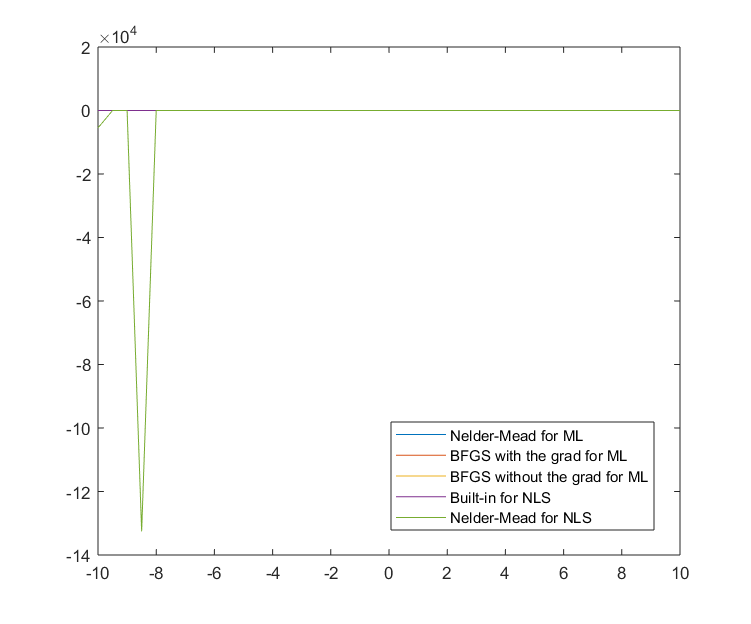
\includegraphics{all5.png}
\caption{Comparison of All the 5}
\end{figure}
Figure 1 shows the estimates for the coefficient for the number of years married $\beta_{2}$. The horizontal axis shows $a$, that is, the values of the initial guess for $\beta_{2}$. We observe the sharp decline around $-8$ for the Nelder-Mead NLS.\par
Figure 2 shows the figure that removes the line for the Nelder-Mead NLS from Figure 1. Function lsqnonlin gives the plausible estimate for only a limited range of the initial guesses around 0 (the purple line).\par
Figure 3 shows the figure that removes the line for the lsqnonlin NLS. Up to $-0.5$, the estimate from the BFGS ML is more stable than that from the Nelder-Mead ML. But above 0.5, the estimate from the BFGS goes away from the seemingly decent estimate 0.12.\par
Figure 4 compares the estimate from the Nelder-Mead ML and those from the BFGS ML (with the analytical gradient). Now I see that the estimates from the BFGS with the analytical gradient for the ML and those from the BFGS without the analytical gradient are the same for the coefficient for the years married $\beta_{2}$.\par
Table 1 shows the computation time for each method. The 2nd column shows the time to compute all the estimates for the initial guesses $(\log(\bar{y}), 0, a, 0, 0, 0)$, where $a$ takes values in [-10:0.5:10]. The BFGS without the analytical gradient was the fastest, and that with the analytical gradient was the slowest. The reason is that in my code in each step of the for loop, the function defining the likelihood and the gradient reads the data $X, y$. This is purely to avoid errors, for otherwise I got an error (when I defined a function for the data and beta and redefined the function for beta in the main file HW3.m).\par
Figure 5 compares the estimate for the coefficient for the constant $\beta_{0}$ from the Nelder-Mead ML and the BFGS ML. The BFGS is more stable locally.\par
Overall, the BFGS is better preferred to the ML by the Nelder-Mead for the local stability and the computation time. But as shown in Figure 4 shows, it does not work very well in some region of initial guesses. My ranking is: ML by BFGS$>$ML by Nelder Mead$>$NLS by lsqnonlin$>$NLS by Nelder Mead.

\begin{figure}
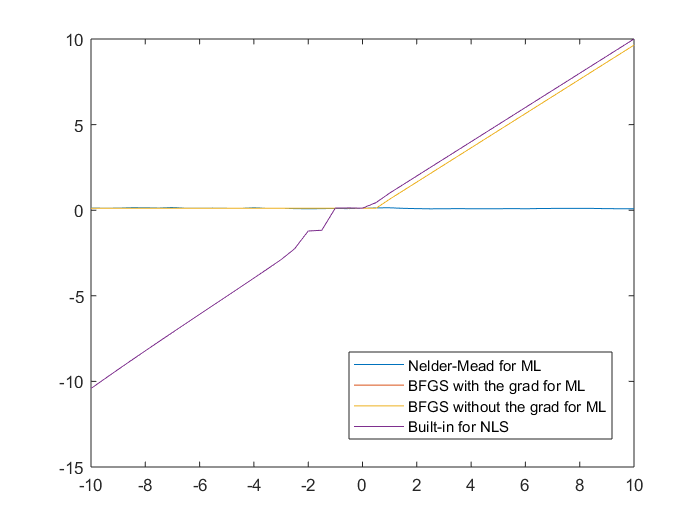
\includegraphics{4.png}
\caption{Comparison of 4}
\end{figure}
\begin{figure}
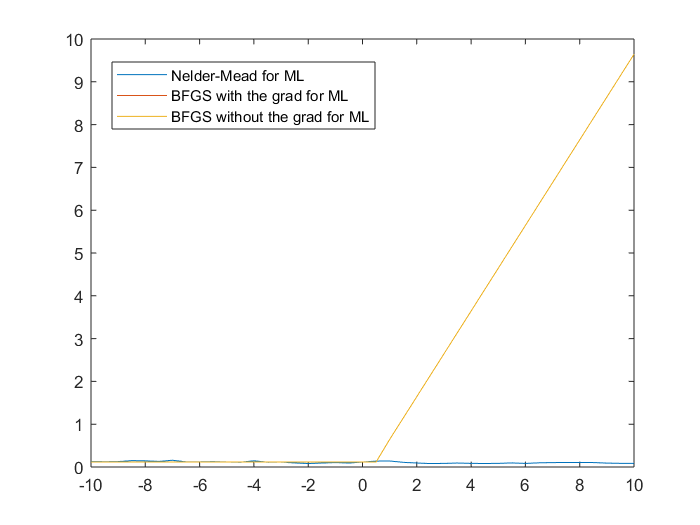
\includegraphics{3.png}
\caption{Comparison of 3}
\end{figure}
\begin{figure}
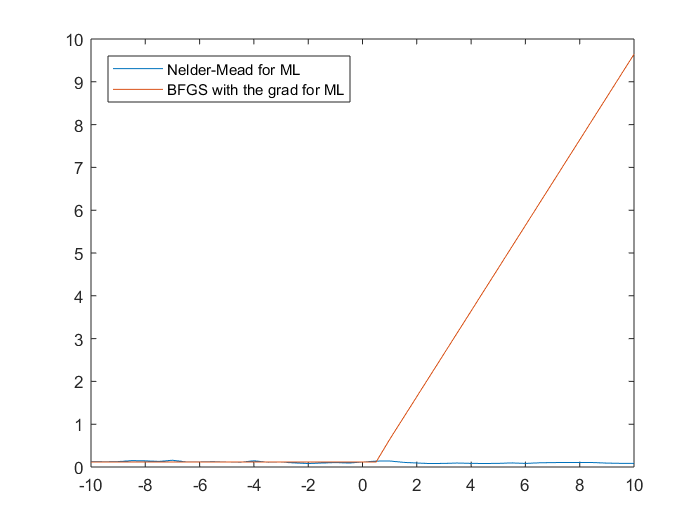
\includegraphics{2.png}
\caption{Comparison of 2}
\end{figure}

\begin{figure}
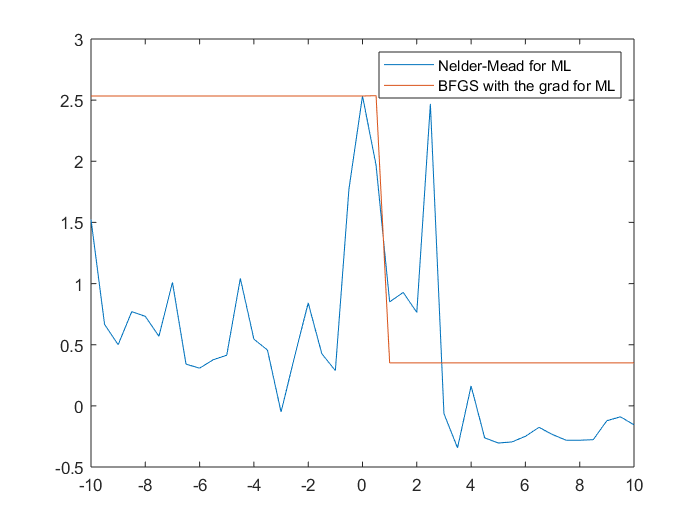
\includegraphics{2_2.png}
\caption{Comparison of 2 for $\hat{\beta}_{0}$}
\end{figure}



\begin{table}[]
\begin{center}
\caption{Computation Time}
\begin{tabular}{lr}
\multicolumn{1}{c}{Method} & \multicolumn{1}{c}{Time (Seconds)} \\
Nelder-Mead, ML            & 1.756                              \\
BFGS with grad, ML         & 3.096                              \\
BFGS without grad, ML      & 0.969                              \\
lsqnonlin                  & 2.179                              \\
Nelder-Mead for NLS        & 0.938                             
\end{tabular}
\end{center}
\end{table}

\clearpage
\question{6}{Code}
The following is copied from HW3.m.
\begin{tiny}
\begin{verbatim}
% Motoaki Takahashi
% HW3 for Econ 512 Empirical Method

clear
diary hw3.out

% x is the n by 6 matrix (explanatory), y is the n by 1 vector (explained)

%% Question 1

load('hw3.mat');
% we have X and y

% write the negative likelihood function as a function of a parameter
loglf_beta = @(beta) -loglf(X,y,beta)

% set the initial guess
beta = [log(mean(y)); zeros(5,1)];

[est_nm, valnm] = fminsearch(loglf_beta, beta)

%% Question 2

% I use the BFGS method.
% the function loglfgrad contains the objective function and the gradient

options = optimoptions('fminunc','Algorithm','quasi-newton',...
          'SpecifyObjectiveGradient',true, 'Display','iter', 'MaxFunctionEvaluations', 30000, 'MaxIterations', 10000);
[est_BFGS, valBFGS] = fminunc('loglfgrad', beta, options)
disp(est_BFGS);

% I calculate the BFGS outcome without the analytical gradient as well

[est_BFGS_wog, val_BFGS_wog] = fminunc(loglf_beta, beta)

% See the difference b/w the outcomes with and without the gradient
est_BFGS-est_BFGS_wog

%% Question 3
nls_beta=@(beta) nls(X,y,beta);
options1 = optimoptions(@lsqnonlin, 'MaxFunctionEvaluations', 30000, 'MaxIterations', 10000)
nls_com = lsqnonlin(nls_beta, beta, -Inf, +Inf, options1)

%% Question 4
nls_nm = fminsearch(nls_beta, beta)

%% Question 5

% See what happens if we move the initial guess for the 3rd element (the coefficient for the years married) from
% -10 to 10. The initial guess for beta_0 is log(mean(y)). The others are kept 0.

grid = [-10:0.5:10];

beta_mat = zeros(6, length(grid));

% the initial guess for beta_0 is log(mean(y))
beta_mat(1, [1:length(grid)]) = log(mean(y))*ones(1, length(grid));

beta_mat(3,[1:length(grid)]) = grid;
% 
% %Nelder-Mead for ML
nm_mat = zeros(6, length(grid));
tic
for n=1:length(grid);
    nm_mat([1:6],n) =  fminsearch(loglf_beta, beta_mat([1:6],n));
end
toc
% 
% %BFGS for ML
BFGS_mat = zeros(6, length(grid));
tic
for n=1:length(grid);
    BFGS_mat([1:6],n) =  fminunc('loglfgrad', beta_mat([1:6],n), options);
end
toc
% % BFGS for ML without the analytical gradient
BFGS_wog_mat =  zeros(6, length(grid));
tic
for n=1:length(grid);
    BFGS_wog_mat([1:6],n) =  fminunc(loglf_beta, beta_mat([1:6],n));
end
toc



% % %lsqnonlin
nls1_mat = zeros(6, length(grid));
tic
for n=1:length(grid);
    nls1_mat([1:6],n) =  lsqnonlin(nls_beta, beta_mat([1:6],n), -Inf, +Inf, options1);
end
toc
% % 
% % %Nelder-Mead for NLS
nls2_mat = zeros(6, length(grid));
tic
for n=1:length(grid);
    nls2_mat([1:6],n) =  fminsearch(nls_beta, beta_mat([1:6],n));
end
toc

% Draw a figure
% I plot the estimates of beta_3 for each initial guess 
plot(grid, nm_mat(3, [1:length(grid)]), grid, BFGS_mat(3, [1:length(grid)]), grid, BFGS_wog_mat(3, [1:length(grid)]), grid, nls1_mat(3, [1:length(grid)]), grid, nls2_mat(3, [1:length(grid)]))

legend('Nelder-Mead for ML', 'BFGS with the grad for ML', 'BFGS without the grad for ML', 'Built-in for NLS', 'Nelder-Mead for NLS')

% Since the nelder-mead for NLS is exceptionally bad, so plot the others
% separately
plot(grid, nm_mat(3, [1:length(grid)]), grid, BFGS_mat(3, [1:length(grid)]), grid, BFGS_wog_mat(3, [1:length(grid)]), grid, nls1_mat(3, [1:length(grid)]))

legend('Nelder-Mead for ML', 'BFGS with the grad for ML', 'BFGS without the grad for ML', 'Built-in for NLS')

% Plot the first three

plot(grid, nm_mat(3, [1:length(grid)]), grid, BFGS_mat(3, [1:length(grid)]), grid, BFGS_wog_mat(3, [1:length(grid)]))

legend('Nelder-Mead for ML', 'BFGS with the grad for ML', 'BFGS without the grad for ML')

% Plot the first two

plot(grid, nm_mat(3, [1:length(grid)]), grid, BFGS_mat(3, [1:length(grid)]))

legend('Nelder-Mead for ML', 'BFGS with the grad for ML')

diary off
\end{verbatim}
\end{tiny}
\end{document}
